\subsection{The Twin Paradox}
Consider two twins \(A\) and \(B\).
Twin \(A\) stays on Earth (considered to be an inertial frame), and \(B\) travels at a constant speed \(v\) to a distant planet \(P\), then she turns around and returns to Earth.
In the frame of reference of \(A\),
\begin{center}
	\begin{tikzpicture}
		\begin{axis}[
				axis lines = left,
				xlabel = \(x\),
				ylabel = \(ct\),
				xtick=\empty,
				ytick=\empty,
				width=4cm,
				height=10cm,
				xmin=0,
				xmax=2.5,
				ymin=0,
				ymax=5,
			]

			%\fill (axis cs:2,1) circle[radius=2pt];
			\node[anchor=south] at (axis cs:1,0) {\(P\)};
			\node[anchor=west] at (axis cs:1,2) {\(E\)};
			\node[anchor=west] at (axis cs:0,4) {\(F\)};
			\draw[dashed,color=lightgray] (axis cs: 1, 0) -- (axis cs: 1, 5);

			\draw[->-=0.5] (axis cs: 0, 0) -- (axis cs: 1, 2);
			\draw[->-=0.5] (axis cs: 1, 2) -- (axis cs: 0, 4);
		\end{axis}
	\end{tikzpicture}
\end{center}
\(E\) is the point where \(B\) reaches \(P\).
The event \(E\) occurs at time \(T\) as perceived by \(A\), so \(E\) has coordinates \((x, ct) = (vT, cT)\).
The time experienced by \(B\) on her outward journey is
\[
	T' = \gamma\qty(T - \frac{v}{c}\cdot vT) = \frac{T}{\gamma}
\]
On her return to event \(F\), twin \(A\) has aged by \(2T\) but twin \(B\) has aged by \(2T' < 2T\).
However, from twin \(B\)'s perspective, twin \(A\) has aged less than she has, since the problem is seemingly symmetric.
This would be a paradox.
To rectify this, consider the frame of reference of \(B\)'s outward journey.
At \(E\), \(x' = 0\) and \(t' = T / \gamma\).
Consider an event \(G\) simultaneous to \(E\) in the frame of reference of \(S'\).
The blue line is a line of constant \(t'\).
\begin{center}
	\begin{tikzpicture}
		\begin{axis}[
				axis lines = left,
				xlabel = \(x\),
				ylabel = \(ct\),
				xtick=\empty,
				ytick=\empty,
				width=4cm,
				height=10cm,
				xmin=0,
				xmax=2.5,
				ymin=0,
				ymax=5,
			]

			%\fill (axis cs:2,1) circle[radius=2pt];
			\node[anchor=south] at (axis cs:1,0) {\(P\)};
			\node[anchor=north west] at (axis cs:1,2) {\(E\)};
			\draw[dashed,color=lightgray] (axis cs: 1, 0) -- (axis cs: 1, 5);
			\draw[color=blue] (axis cs: 0, 1.75) -- (axis cs: 2, 2.25);
			\node[blue,anchor=north west] at (axis cs:0,1.75) {\(G\)};

			\draw[->-=0.5] (axis cs: 0, 0) -- (axis cs: 1, 2);
			\draw[->-=0.5] (axis cs: 1, 2) -- (axis cs: 0, 4);
		\end{axis}
	\end{tikzpicture}
\end{center}
At \(E\),
\[
	t' = \gamma\qty(t - \frac{vx}{c^2}) = t\gamma \implies t = \frac{t'}{\gamma} = \frac{T}{\gamma^2}
\]
So each of them thinks that the other has aged less, when \(B\) is at \(E\), by a factor of \(\gamma^{-1}\).
On the return,
\begin{center}
	\begin{tikzpicture}
		\begin{axis}[
				axis lines = left,
				xlabel = \(x\),
				ylabel = \(ct\),
				xtick=\empty,
				ytick=\empty,
				width=4cm,
				height=10cm,
				xmin=0,
				xmax=2.5,
				ymin=0,
				ymax=5,
			]

			%\fill (axis cs:2,1) circle[radius=2pt];
			\node[anchor=south] at (axis cs:1,0) {\(P\)};
			\node[anchor=west,xshift=0.4cm] at (axis cs:1,2) {\(E\)};
			\draw[dashed,color=lightgray] (axis cs: 1, 0) -- (axis cs: 1, 5);
			\draw[color=red] (axis cs: 0, 2.25) -- (axis cs: 2, 1.75);
			\node[red,anchor=south west] at (axis cs:0,2.25) {\(H\)};
			\draw[color=blue] (axis cs: 0, 1.75) -- (axis cs: 2, 2.25);
			\node[blue,anchor=north west] at (axis cs:0,1.75) {\(G\)};

			\draw[->-=0.5] (axis cs: 0, 0) -- (axis cs: 1, 2);
			\draw[->-=0.5] (axis cs: 1, 2) -- (axis cs: 0, 4);
		\end{axis}
	\end{tikzpicture}
\end{center}
The red line is a line of constant \(t'\) as measured by \(B\) on the return journey, at \(E\).
So for the return journey, \(A\) sees \(B\) age from the event \(E\) to the event \(F\).
However, \(B\) sees \(A\) age from the event \(H\) to the event \(F\).
So there is a time gap between \(G\) and \(H\) as observed by \(B\), which is not considered by the naive model of this problem.
\(B\) sees \(A\) age instantaneously at the point when she changes direction.
In particular, the frame of \(B\) as she changes direction is not inertial.

\subsection{Length Contraction}
The length of an object is dependent on the choice of frame.
Consider a rod of length \(L'\) in \(S'\), which is stationary in \(S'\).
The world lines of the ends of the rod are vertical.
The length of the rod at time \(t'\) is the distance in \(x'\) between the two world lines.
In \(S\),
\[
	x' = 0 \implies \gamma(x - vt) = 0
\]
Further,
\[
	x' = L' \implies \gamma(x - vt) = L'
\]
Therefore, the distance between the two \(x\) points at the same \(t\) is \(L = L'/\gamma < L'\).
So the length of a moving object shrinks in the direction it is moving.
Sometimes, analogously to `proper time', we consider the `proper length' of an object, which is the length as measured in the rest frame of the object.

For example, does a train of (proper) length \(2L\) fit alongside a platform of length \(L\) if it is travelling along the tracks at a speed such that \(\gamma = 2\)? For observers on the platform, the train indeed contracts to length \(L\), so indeed it fits.
On the other hand, for observers on the train, the platform contracts to a length \(\frac{1}{2}L\), so the train would not fit.
To resolve the uncertainty, we will draw a spacetime diagram, from the frame of reference \(S\) where the platform is stationary.
The red lines represent the end points of the platform.
The world lines for the end points of the train are in blue.
\(E\) is the event when the rear of the train is at the rear of the platform, and \(F\) is the event where the front of the train is at the front of the platform.
\begin{center}
	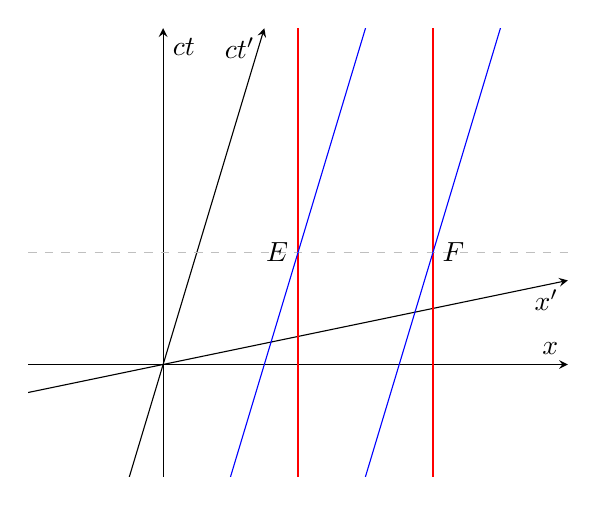
\begin{tikzpicture}
		\begin{axis}[
				axis lines = center,
				xlabel = \(x\),
				ylabel = \(ct\),
				xtick=\empty,
				ytick=\empty,
				xmin=-1,
				xmax=3,
				ymin=-1,
				ymax=3,
			]

			\draw[->,>=stealth] (axis cs: -0.5, -2) -- (axis cs: 0.75, 3);
			\node[anchor=north east] at (axis cs:0.75,3) {\(ct'\)};
			\draw[->,>=stealth] (axis cs: -2, -0.5) -- (axis cs: 3, 0.75);
			\node[anchor=north east] at (axis cs:3,0.75) {\(x'\)};

			\draw[color=red] (axis cs: 1, -1) -- (axis cs: 1, 3);
			\draw[color=red] (axis cs: 2, -1) -- (axis cs: 2, 3);

			\draw[dashed,color=lightgray] (axis cs: -1, 1) -- (axis cs: 3, 1);
			\node[anchor=east] at (axis cs:1, 1) {\(E\)};
			\node[anchor=west] at (axis cs:2, 1) {\(F\)};

			\draw[color=blue] (axis cs: 0, -3) -- (axis cs: 2, 5);
			\draw[color=blue] (axis cs: 1, -3) -- (axis cs: 3, 5);

			%\draw[dashed,color=lightgray] (axis cs: 1, 0) -- (axis cs: 2, 5);
		\end{axis}
	\end{tikzpicture}
\end{center}
Let \(E\) correspond to \(t = 0\) and \(t' = 0\).
The front of the train is at \(x' = 2L\), and the front of the platform is at \(x = L\).
In the \(S\) frame, events \(E\) and \(F\) occur at the same time \(t = 0\).
\[
	x' = \gamma(x - vt) \implies 2L = \gamma(L - vt) = 2(L - vt) \implies t = 0
\]
Further,
\[
	x = \gamma(x' + vt') \implies L = \gamma(2L + vt') = 2(2L + vt') \implies t' = \frac{L - 4 L}{2v} = \frac{-3L}{2v} < 0
\]
Hence, the time \(t'\) at which \(F\) occurs is before the event \(E\).
So from the perspective of the train, the front of the train has already passed the front of the platform by the time that the back of the train passes the back of the platform, so from this perspective the train does not fit.
